%\documentclass[a4paper]{article}
%\usepackage{beamerarticle}
%\documentclass[handout]{beamer}
%\usepackage{handoutWithNotes}
%\setbeameroption{show notes} 
%\pgfpagesuselayout{4 on 1 with notes}[a4paper,border shrink=5mm]
%\documentclass[ignorenonframetext,red]{beamer}

%\documentclass[notes=only]{beamer} %notes only
% \documentclass[notes]{beamer} %slides with notes
\documentclass{beamer}

\mode<presentation>{
	% \usetheme{Goettingen}
	\usetheme{CambridgeUS} 
	\usecolortheme{beaver}
	%\setbeamercovered{transparent}
}

%set up chinese environment
\usepackage{fontspec}
\newfontfamily\zhfont[BoldFont=Hiragino Sans GB W3]{Hiragino Sans GB W3} %设置中文
\newfontfamily\zhpunctfont{Hiragino Sans GB W3} % 设置中文
\XeTeXlinebreaklocale "zh"
\XeTeXlinebreakskip = 0pt plus 1pt
\renewcommand{\today}{\number\year 年\number\month 月\number\day 日}
% \setmainfont{Hiragino Sans GB W3}           %这里设置英文衬线字体
% \setmonofont{Hiragino Sans GB W3}                     %英文等宽字体
% \setsansfont{Hiragino Sans GB W3}               %英文无衬线字体
\usepackage{zhspacing}
\zhspacing

% set up other environment
\usepackage[english]{babel}
\usepackage[utf8]{inputenc}
\usepackage{graphicx}
\usepackage{times}
\usepackage[T1]{fontenc}
\usepackage{animate}
% \usepackage[caption=false,font=footnotesize]{subfig}
\usepackage[font=footnotesize]{subfig}
\usepackage{listings}
\lstset{language=C++}
\lstset{breaklines}
\lstset{extendedchars=false}
\lstset{basicstyle=\tiny}
\lstset{frame=shadowbox}

\usepackage[justification = centering,labelsep = period,font = scriptsize]{caption}
\setlength{\abovecaptionskip}{1pt}
\setlength{\belowcaptionskip}{1pt}
\usepackage{amssymb}
\usepackage{epstopdf}
% for pseudo codes
\usepackage{float}
\usepackage{algorithm}
\usepackage{algorithmicx}
\usepackage{algpseudocode}
\usepackage{tikz}
\usetikzlibrary{arrows,calc,intersections}
\usetikzlibrary{shapes.callouts}
\tikzset{
	level/.style   = { ultra thick, blue },
	connect/.style = { dashed, red },
	notice/.style  = { draw, rectangle callout, callout relative pointer={#1} },
	label/.style   = { text width=2cm }
}
\usepackage{xcolor}
\makeatletter


\newcommand\tikzmark[1]{%
	  \tikz[overlay,remember picture,baseline] \coordinate (#1);}

\setbeamertemplate{footline}[frame number]

\title{基于Intel Xeon/Xeon Phi平台的关于离散时间对冲误差的并行化研究}

\logo{
  
\includegraphics[width=0.4cm,height=0.4cm,keepaspectratio]{Figures/logo-MdS.jpg}%
  \hspace{0.5ex}
  
\includegraphics[width=0.4cm,height=0.4cm,keepaspectratio]{Figures/logo-CEA.jpg}%
  \hspace{0.5ex}
  
\includegraphics[width=0.6cm,height=0.8cm,keepaspectratio]{Figures/logo-cnrs2.png}%
  \hspace{0.5ex}
  
\includegraphics[width=0.4cm,height=0.35cm,keepaspectratio]{Figures/logo-versaille2.png}%
}

\institute[机构1,机构2, 机构3] % (optional, but mostly needed)
{
  \inst{1} Maison de la Simulation 
  \and
  \inst{2} Atomic Energy and Alternative Energies Commission (C.E.A) 
  \and
  \inst{3} French National Centre for Scientific Research (C.N.R.S) 
  \and
  \inst{4} Versailles Saint-Quentin-en-Yvelines University \\ 
  \vspace{3ex}
  \scalebox{4}{\insertlogo}
}

\author[作者] % (optional, use only with lots of authors)
{\scriptsize 叶帆\inst{1,2} \and 陈浪石\inst{1,3} \and 潘慈辉\inst{1,4}}

% % - Keep it simple, no one is interested in your street address.
%
% \only<presentation>{
%
%   \subject{Krylov Subspace, Auto-tuning, Arnoldi Orthogonalization}
% }

% \pgfdeclareimage[height=0.5cm]{university-logo}{university-logo-filename}
% \logo{\pgfuseimage{university-logo}}

% Delete this, if you do not want the table of contents to pop up at
% the beginning of each subsection:

\AtBeginSection[]
{
	\begin{withoutheadline}
		\begin{frame}<beamer>{内容提要}
			\tableofcontents[currentsection,currentsubsection]
		\end{frame}
	\end{withoutheadline}
}

% If you wish to uncover everything in a step-wise fashion, uncomment
% the following command: 
%\beamerdefaultoverlayspecification{<+->}

\makeatletter
\newenvironment{withoutheadline}{
  \setbeamertemplate{headline}[default]
  \def\beamer@entrycode{\vspace*{-\headheight}}
}{}
\makeatother
\setbeamertemplate{navigation symbols}{}
\setbeamertemplate{footline}[pagenumber]

\begin{document}

\begin{frame}[plain]
	\titlepage
\end{frame}

%remove logs at footline of each page
\setbeamertemplate{logo}{}

\begin{withoutheadline}
\begin{frame}
	\frametitle{内容提要}
	% \tableofcontents[hideothersubsections]
	\tableofcontents
	\note[item]{注释说明1}
\end{frame}
\end{withoutheadline}

\section{背景介绍} % (fold)
\label{sec:context}

\begin{withoutheadline}
\begin{frame}
	\frametitle{超算发展及Xeon Phi}
	\vspace{-4ex}
	\begin{columns}
		\begin{column}[T]{0.4\textwidth}
			高性能计算已经进入后Petaflop($10^{15}$)时代。但是能优化到Petaflop级别的实际应用却很少,面临问题如下
				\vspace{1ex}
			\begin{itemize}
				\item 算法的内在并行性不足
				\vspace{1ex}
				\item 并行算法的通信受制于内存和网络连接
				\vspace{1ex}
				\item 并行编程的难度
			\end{itemize}
			\vspace{1ex}
			超级计算机本身还面临
			\begin{itemize}
				\item 能耗过大
			\end{itemize}
		\end{column}\hfill
		\begin{column}[T]{0.6\textwidth}
				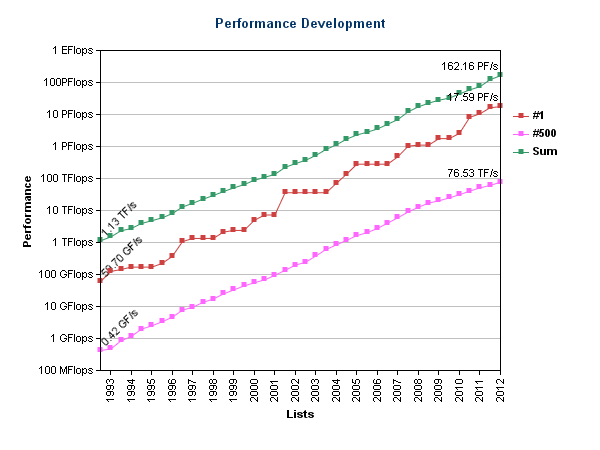
\includegraphics[width=\textwidth]{Figures/context/top500Perf.png}
				\begin{center}
					\scriptsize
					超算Top500发展趋势
				\end{center}
		\end{column}
	\end{columns}
\end{frame}
\end{withoutheadline}

\begin{withoutheadline}
\begin{frame}
	\frametitle{超算发展及Xeon Phi}
	\begin{columns}
		\begin{column}[T]{0.4\textwidth}
			单个CPU的发展已经达到性能和功耗的瓶颈,超算转向众核架构(Manycore), 其具有如下优势
			\begin{itemize}
				\item 高带宽(bandwidth)带来的高通量(high data throughput)
				\item 高能耗效率(flops/watt)
					\note[item]{世界绿色500强榜单上的高能效机器越来越多采用众核结构}
				\item 适合大规模的数据并行性应用(data parallel)
			\end{itemize}
			目前众核结构处理器的代表
			\begin{itemize}
				\item Nvidia 的GPU加速器
				\item Intel 的Xeon Phi协处理器
			\end{itemize}
		\end{column}\hfill
		\begin{column}[T]{0.6\textwidth}
			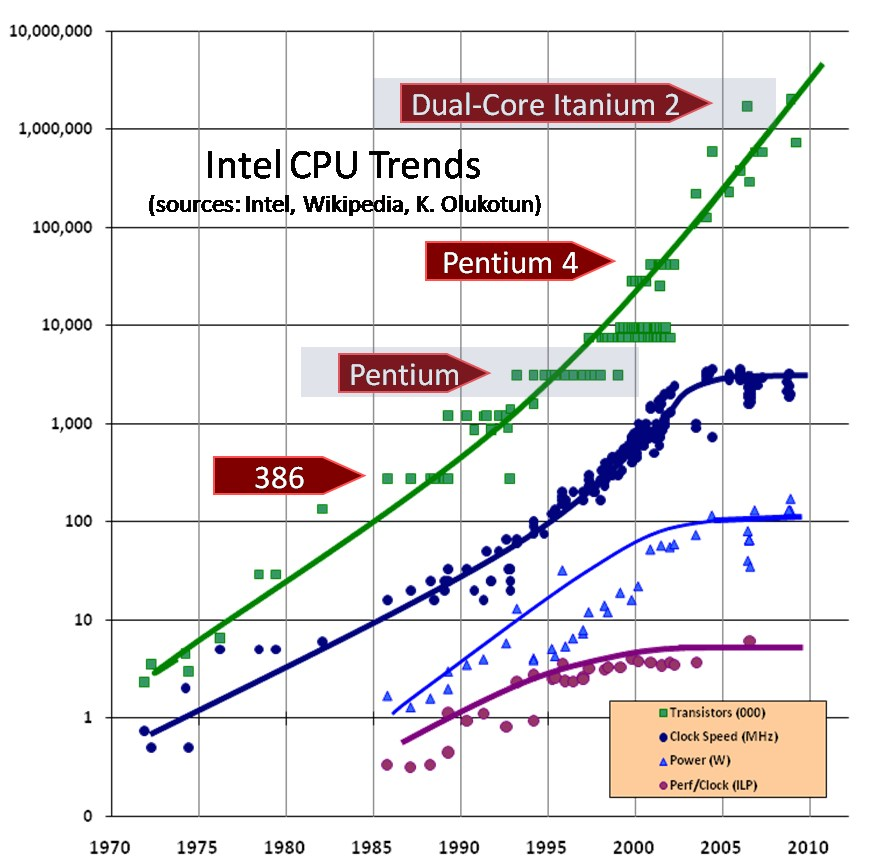
\includegraphics[width=\textwidth]{Figures/context/CPU-Scaling.jpg}
			\begin{center}
				\scriptsize
				单个CPU发展遇到的各种瓶颈问题
			\end{center}
		\end{column}
	\end{columns}
\end{frame}
\end{withoutheadline}

\begin{withoutheadline}
	\begin{frame}
		\frametitle{金融领域的超算}
			\vspace{-1em}
			\begin{center}
			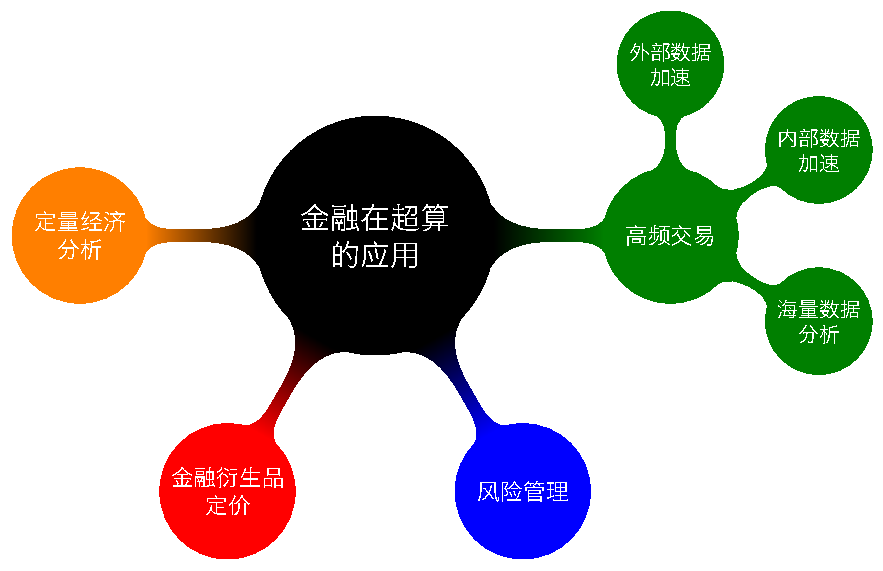
\includegraphics[width=\textwidth]{Figures/context/tikz/finance-hpc.pdf}
			\end{center}
			\begin{center}
				金融在高性能计算上的几大应用
			\end{center}
	\end{frame}
\end{withoutheadline}

\begin{withoutheadline}
	\begin{frame}[t]
		\frametitle{金融领域的超算}
		\begin{columns}
			\begin{column}[T]{0.48\textwidth}
			\begin{block}{高频交易}
				从那些人们无法利用的极为短暂的市场变化中寻求获利的计算机化交易
			\end{block}
			\begin{enumerate}
				\item 数据在交易所和计算机之间加速(co-location)
				\item 数据在计算机内部加速(网卡+CPU 或者 FPGA
				\item 海量数据的分析工作
			\end{enumerate}
		\end{column}\hfill
		\begin{column}[T]{0.48\textwidth}
			\begin{block}{金融衍生品定价}
				衍生品的复制与对冲策略,以减少最终收益的不确定性
			\end{block}
			\begin{itemize}
				\item 模型的复杂度带来了密集的计算量
				\item 对冲的时效性需要计算的高速性 
			\end{itemize}
		\end{column}
		\end{columns}
		\vspace{2ex}
		\begin{center}
			金融交易越来越依赖计算机程序和高性能计算集群
		\end{center}
	\end{frame}
\end{withoutheadline}

% section 背景介绍 (end)

\section{课题陈述} % (fold)
\label{sec:subject}

\begin{withoutheadline}
\begin{frame}
	\frametitle{欧式期权}
	content	
\end{frame}
\end{withoutheadline}

\begin{withoutheadline}
\begin{frame}
	\frametitle{Black-Scholes模型}
	content
\end{frame}
\end{withoutheadline}

\begin{withoutheadline}
\begin{frame}
	\frametitle{对冲策略及误差分析}
	content
\end{frame}
\end{withoutheadline}
% section 课题陈述 (end)

\begin{withoutheadline}
\begin{frame}
	\frametitle{参数选择及收敛条件}
	content	
\end{frame}
\end{withoutheadline}

\section{并行化算法} % (fold)
\label{sec:algorithm}

\begin{withoutheadline}
\begin{frame}
	\frametitle{常用的并行化策略}
	\begin{columns}
		\begin{column}[T]{0.48\textwidth}
			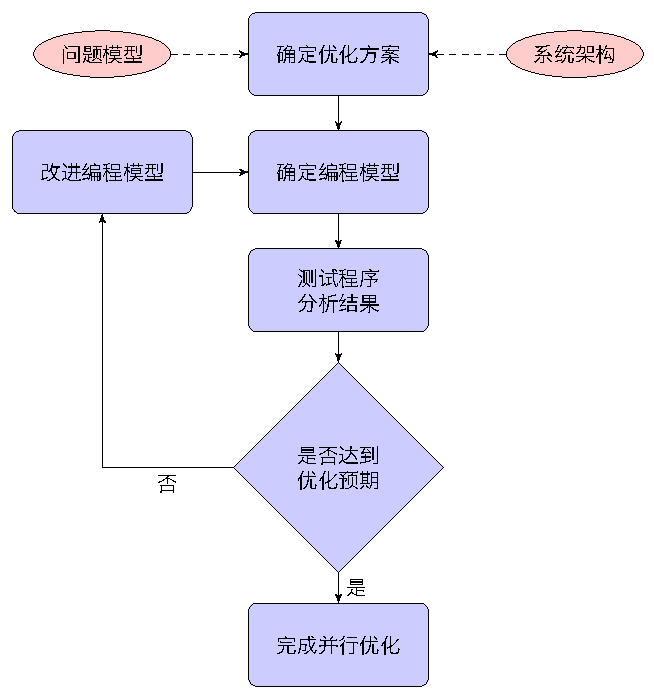
\includegraphics[width=\textwidth]{Figures/algorithm/tikz/flowchart1.pdf}
		\end{column}\hfill
		\begin{column}[T]{0.48\textwidth}
				 针对内存使用的优化
					\begin{itemize}
						\item 对齐数据(data alignment)
						\item 数据块(cache blocking)
						\item 预读取(prefetching)
						\item 流式存储技术(streaming store)
					\end{itemize}
				 针对for循环的改进
					\begin{itemize}
						\item 循环展开(loop unrolling)
						\item 分块循环(loop tiling)
						\item 循环互换(loop interchange)
						\item 循环合并(loop fusion)
						\item 循环偏移(loop skewing)
						\item 循环剥离(loop peeling)
					\end{itemize}
		\end{column}
	\end{columns}
	\end{frame}
\end{withoutheadline}


\begin{withoutheadline}
\begin{frame}[fragile]
	\frametitle{算法并行性分析}
	\begin{algorithmic}
  \tiny
	 % \Require $X_0$ \Comment{金融产品在$t=0$时的初始价格}
	 % \Require $\sigma$ \Comment{市场波动性}
	 % \Require $K$ \Comment{期权合约价格}
	 % \Require $T$ \Comment{期权到期时间}
	 % \Require $\epsilon$ \Comment{可接受的误差上限}
     %     \Require $M$ \Comment{蒙特卡洛模拟次数}
     %     \Require $N$ \Comment{离散抽样次数}
     %     \Ensure $prob$
	 \Procedure{BSERROR}{M, N}
         \State $error \gets 0$ %\Comment{离散策略和连续策略的误差}
         \State $NRV[N]$ %\Comment{符合正态分布的N个独立随机数}
         \State $BM[N]$ %\Comment{布朗运动的N个状态}
         \State $PX[N+1]$ %\Comment{在离散时间点的期权价格}
	 \State $\delta t \gets T/N$ %\Comment{时间间隔}
	 \State\tikzmark{start1} $count \gets 0$ %\Comment{在$M$次模拟中$N$被接受的次数}
	  \For{$m=1:M$}\tikzmark{end1} %\Comment{M次蒙特卡洛模拟}
      \State\tikzmark{start2}$error \gets 0$ %\Comment{离散策略和连续策略的误差}
	  \ForAll {$NRV[j]$}\tikzmark{end2}
	     $NRV[j] \gets GaussianNumGenerator()$
	  \EndFor    
	  \State \tikzmark{start3}$BM[0] \gets NRV[0] \cdot \sqrt{\delta t}$ 
	  \ForAll {$BM[j]$}\tikzmark{end3}
	     $BM[j] \gets BM[j-1] + NRV[j]\cdot \sqrt{\delta t}$ 
	  \EndFor
	  \State \tikzmark{start4}$PX[0] \gets X0$
	  \ForAll {$j= 1:N+1$}\tikzmark{end4}
	  \State $PX[j]\gets X0 \cdot exp(-0.5\cdot \sigma^2 \cdot j \cdot \delta t + \sigma \cdot BM[j-1])$
	  \EndFor
	  \tikzmark{start5}\ForAll{$j=0:N-1$}\tikzmark{end5}
	  \State $Upper \gets (\log(PX[j]/K) + 0.5\cdot \sigma^2 \cdot (T- T_j))/ (\sigma \cdot \sqrt{T-T_j})$ 
	  \State $error \gets error - 1/(\sqrt{2\pi}) \cdot (PX[j+1]-PX[j])\cdot \int_{-\infty}^{Upper}e^{-t^2/2}dt $
	  \EndFor
	  % \If {$PX[N] > K$} 
	  % \State $error \gets error + (PX[N]-K)$
	  % \EndIf
	  % \State $Upper1 \gets (log(X0/K) + 0.5\cdot \sigma^2 \cdot T)/(\sigma \sqrt{T})$
	  % \State $Upper2 \gets (log(X0/K) - 0.5\cdot \sigma^2 \cdot T)/(\sigma \sqrt{T})$
	  % \State $error = error + K/\sqrt{2\pi} \cdot \int_{-\infty}^{Upper2}e^{-t^2/2}dt -X0/\sqrt{2\pi}\cdot \int_{-\infty}^{Upper1}e^{-t^2/2}dt$
	  % \If {$error < \epsilon$} 
	  % \State $count \gets count + 1$ 
	  % \EndIf
	  \EndFor
	  % \State $prob \gets count/M$
	  % \State return $prob$
	 \EndProcedure
  \end{algorithmic}\vfill
  \pause
  \begin{tikzpicture}[remember picture,overlay]
	  \draw[blue, thick] ( $ (start1) + (-2pt,-2pt) $ ) rectangle ( $ (end1) + (2pt,-2pt)$ );
      \pause
	  \draw[red, thick] ( $ (start2) + (-2pt,-2pt) $ ) rectangle ( $ (end2) + (2pt,-2pt)$ );
	  \draw[red, thick] ( $ (start3) + (-2pt,-2pt) $ ) rectangle ( $ (end3) + (2pt,-2pt)$ );
	  \draw[red, thick] ( $ (start4) + (-2pt,-2pt) $ ) rectangle ( $ (end4) + (2pt,-2pt)$ );
	  \draw[red, thick] ( $ (start5) + (-22pt,-2pt) $ ) rectangle ( $ (end5) + (2pt,-2pt)$ );
    \pause
	\node[notice={(-3.5cm, -1cm)}, draw=black, text=blue, text width=3cm, align=left, font=\tiny] at ($(end1) + (5cm, 1.5cm)$) { 
			蓝色的外层循环为相互独立的蒙特卡洛模拟次数并行度高, 可并行在单个MIC的不同线程上也可以并行在多个MIC处理器上};
  \pause
	\node[notice={(-4.5cm, 0.4cm)}, draw=black, text=red, text width=3cm, align=left, font=\tiny] at ($(end2) + (6.5cm, -0.5cm)$) { 
			红色循环为离线状态数组, 数组前后状态有依赖关系,需要进行并行优化};
	\end{tikzpicture}
\end{frame}
\end{withoutheadline}

\begin{withoutheadline}
\begin{frame}
	\frametitle{单片MIC单次蒙特卡洛并行优化}
	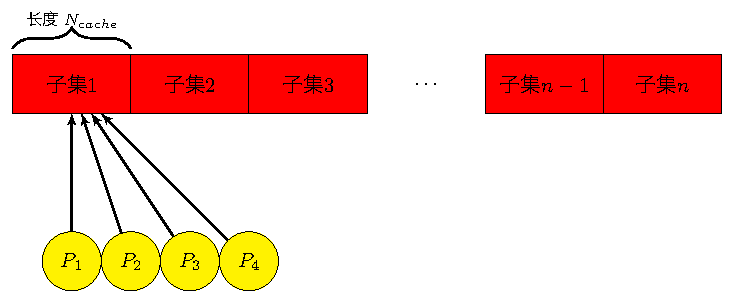
\includegraphics[width=0.9\textwidth]{Figures/algorithm/tikz/sMICOpt.pdf}\vfill
\begin{block}{方案一}
	离线状态的数组总长度N分为$n$个子集,每个的长度为$N_{cache}$, 单片MIC上的所有线程依次同时
	并行工作于子集1, 子集2,直至最后一个子集。$N_{cache}$的大小要和缓存大小匹配,使数据可以在缓存
	内被所有线程所共享($512K \times 61 = 31M$, 所有线程共享一个随机数发生流)
\end{block}
\end{frame}
\end{withoutheadline}

\begin{withoutheadline}
\begin{frame}
	\frametitle{单片MIC单次蒙特卡洛并行优化}
	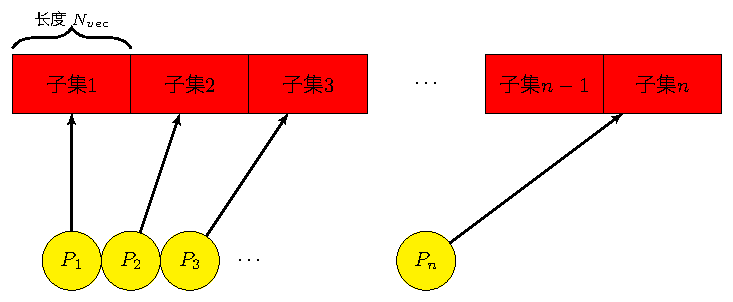
\includegraphics[width=0.9\textwidth]{Figures/algorithm/tikz/sMICOpt2.pdf}\vfill
\begin{block}{方案二}
	离线状态的数组总长度N分为$n$个子集,每个的长度为$N_{vec}$, 每个子集由一个线程负责,所有线程同时
	并行工作,每个线程拥有自己的随机数发生流,$N_{vec}$ 要和单个核心的$L2$缓存相符合(512K),以达到最大的数据重用。
\end{block}
\end{frame}
\end{withoutheadline}

\begin{withoutheadline}
\begin{frame}
	\frametitle{基于汇编的矢量化积分运算}
	并行算法中大量使用了如下形式的积分运算
	\begin{block}{}
		\begin{equation}
			f(x)=\int_{-\infty}^{x}e^{-\frac{t^2}{2}}dt
		\end{equation}
	\end{block}
	利用辛普森积分法(Simpson's rule)可以对高斯积分进行矢量化(vectorized)计算
	\begin{block}{转化为高斯积分}
		\begin{equation}
			\label{eq:gauss}
			f(x)=\int_{-\infty}^{x}e^{-\frac{t^2}{2}}dt=0.5\times \sqrt{2\pi} + \int_{0}^{x}e^{-\frac{t^2}{2}}dt
		\end{equation}
	\end{block}
	\begin{block}{Simpson's rule}
		\begin{equation}
			\label{eq:simpson}
			\int_{a}^{b}f(x)dx\approx \frac{h}{3}\left[f(x_0)+2\sum\limits_{j=1}^{n/2-1}f(x_{2j})+4\sum\limits_{j=1}^{n/2}f(x_{2j-1})+f(x_n)\right]
		\end{equation}
	\end{block}
\end{frame}
\end{withoutheadline}

\begin{withoutheadline}
\begin{frame}
	\frametitle{基于二分法的N值最优化搜索}
	\begin{columns}
		\begin{column}[T]{0.5\textwidth}
			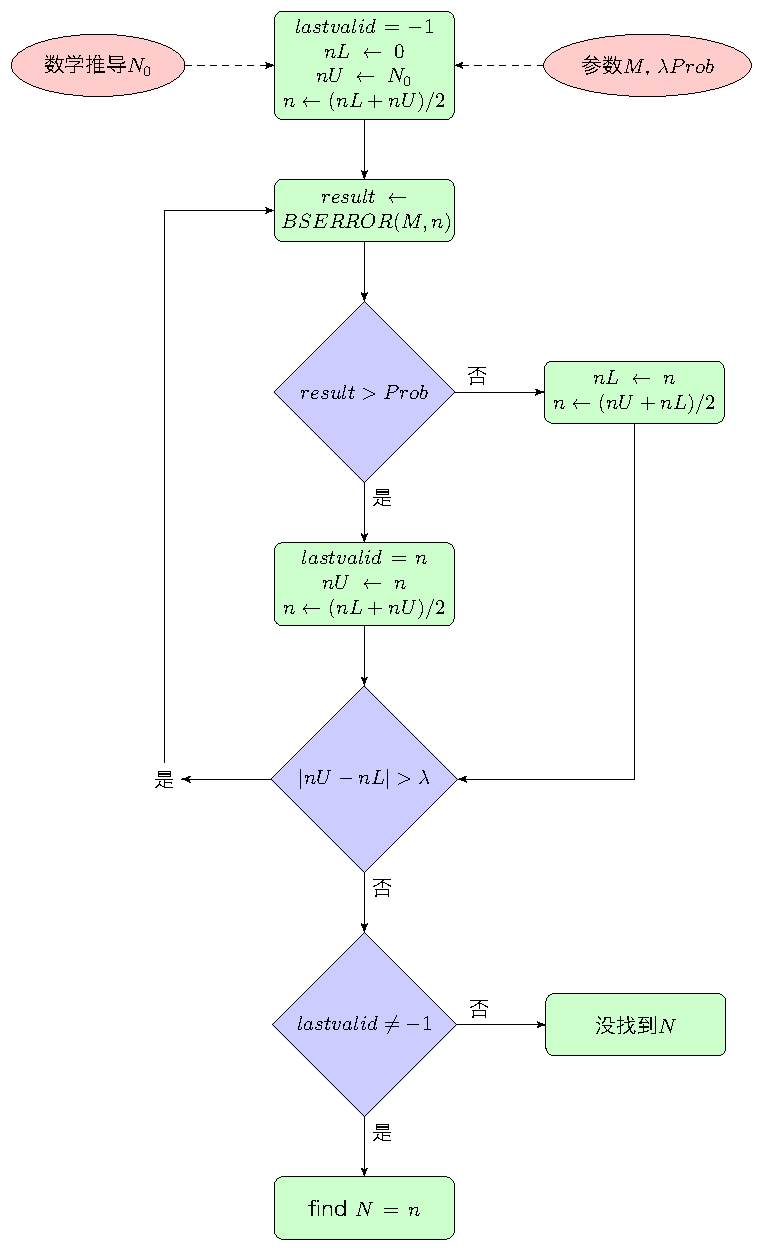
\includegraphics[width=0.8\textwidth]{Figures/algorithm/tikz/flowchart2.pdf}
		\end{column}\hfill
		\begin{column}[T]{0.5\textwidth}
			\begin{block}{初始值$N_0$}
				本文通过数学推导给出了一个$N$值的上界$N_0$, 从而使我们的二分法有了初始的
				搜索上界
			\end{block}
			\begin{block}{参数$\lambda$, $Prob$, $M$}
				$\lambda$是设置的最小区间,当上下界之差小于$\lambda$时,认为二分法结束
				$Prob$则为置信概率,值越高表明最后搜索到得$N$值可信度越高。
				$M$为蒙特卡洛模拟的次数,越大的$M$也说明搜索到的结果越可靠。
			\end{block}
		\end{column}
	\end{columns}
\end{frame}
\end{withoutheadline}

\begin{withoutheadline}
\begin{frame}
	\frametitle{多MIC并行优化}
	\vspace{-1ex}
	\begin{block}{Maser-Slave模式}
		一个节点被选为Master,其余节点为Slave节点在$M$的维度上进行并行优化。
	\end{block}
	\begin{center}
		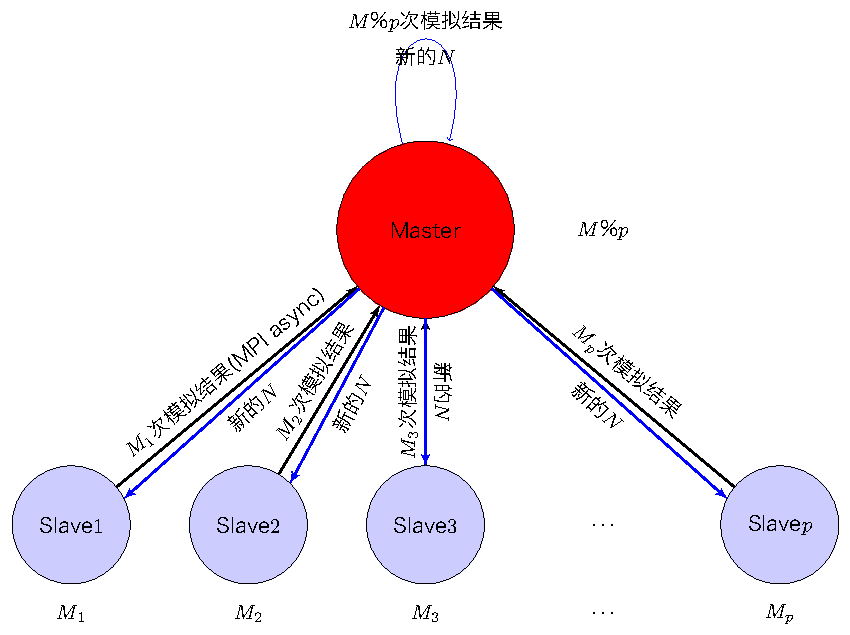
\includegraphics[width=0.7\textwidth]{Figures/algorithm/tikz/mBSERROR.pdf}
	\end{center}
\end{frame}
\end{withoutheadline}

% section 并行化算法 (end)

\section{实验结果及分析} % (fold)
\label{sec:exp}

\begin{withoutheadline}
	\begin{frame}
		\frametitle{单MIC及CPU版本的实验对比(1/2)}
		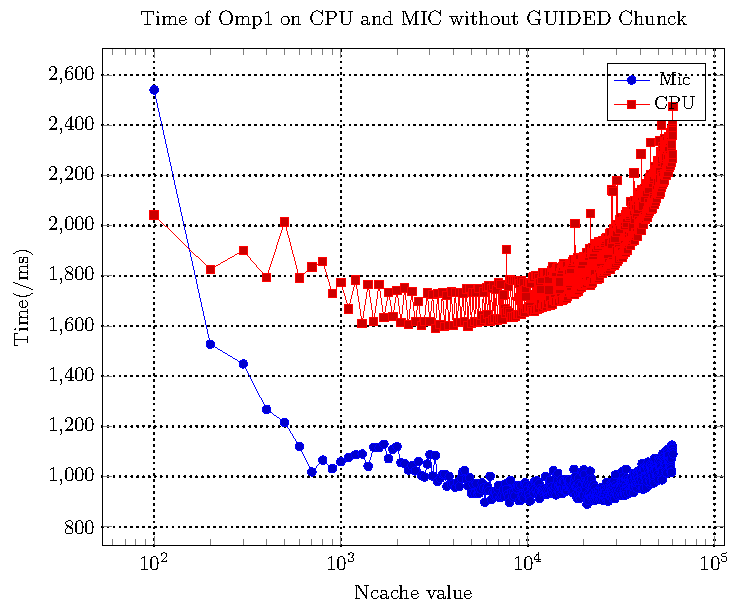
\includegraphics[width=0.8\textwidth]{Figures/exp/bsV1-6-mic-cpu-Time-Chunck-0.pdf}\vfill
		\begin{tikzpicture}[overlay]
			\node[draw=black, text=black,text width=1cm, align=left, font=\tiny] at (10.5,6){
				单机并行算法1在单块CPU和单块MIC上的实验对比,Chunk采用系统默认调度策略};
			\pause
			\node[notice={(-1.6cm, -1.4cm)}, draw=black, text=blue,text width=3cm, align=left, font=\tiny] at (9,3.5) {  
				Ncache值取在$10^4$时MIC运算时间最短,2x加速CPU};
			\pause
			\node[notice={(1cm, -2.4cm)}, draw=black, text=red,text width=3cm, align=left, font=\tiny] at (5,7) {  
				CPU版本也存在Ncache最优区间};
		\end{tikzpicture}
	\end{frame}
\end{withoutheadline}

\begin{withoutheadline}
\begin{frame}
	\frametitle{单MIC及CPU版本的实验对比(2/2)}
	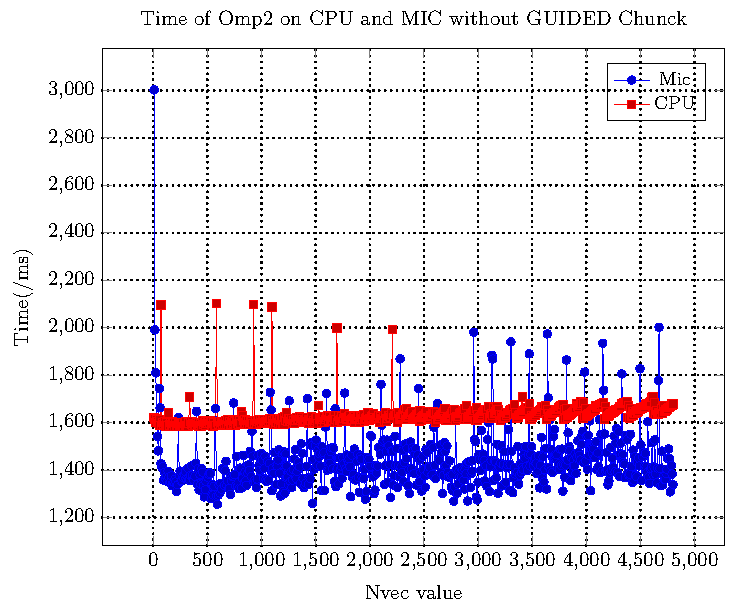
\includegraphics[width=0.8\textwidth]{Figures/exp/bsV2-6-mic-cpu-Time-Chunck-0.pdf}\vfill
		\begin{tikzpicture}[overlay]
			\node[draw=black, text=black,text width=1cm, align=left, font=\tiny] at (10.5,6) {
				单机并行算法2在单块CPU和单块MIC上的实验对比,Chunk采用系统默认调度策略};
			\pause
			\node[notice={(1cm, -3.4cm)},draw=black, text=blue, text width=3cm, align=left, font=\tiny] at (5,6) {
				MIC版本仍有优势,时间随Nvec值变化而小幅度波动,系统Chunk自动调整的结果};
		\end{tikzpicture}
\end{frame}
\end{withoutheadline}

\begin{withoutheadline}
\begin{frame}
	\frametitle{Chunk取值对算法1的影响}
	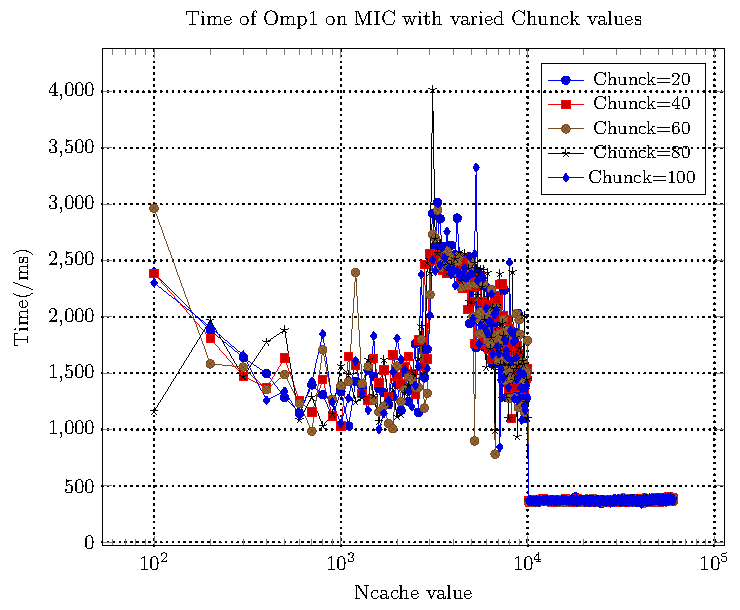
\includegraphics[width=0.8\textwidth]{Figures/exp/bsV1-mic-Time-Chunck.pdf}\vfill
	\begin{tikzpicture}[overlay]
		\node[draw=black, text=black,text width=1cm, align=left, font=\tiny] at (10.5,6){
			Chunk值是系统每次分配给单个线程的并行任务数量, 图为算法1在MIC上的测试取5组不同的Chunk值};
	\end{tikzpicture}
\end{frame}
\end{withoutheadline}

\begin{withoutheadline}
\begin{frame}
	\frametitle{Chunk取值对算法2的影响}
	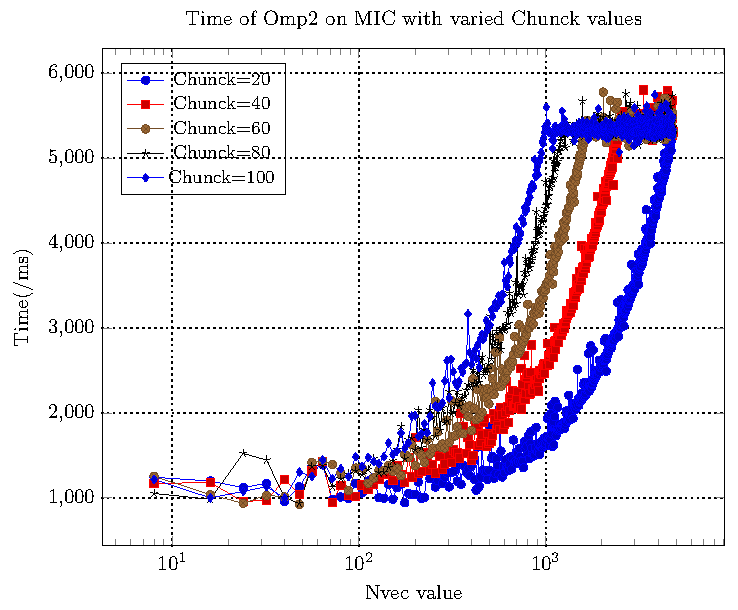
\includegraphics[width=0.8\textwidth]{Figures/exp/bsV2-mic-Time-Chunck.pdf}\vfill
		\begin{tikzpicture}[overlay]
			\node[draw=black, text=black,text width=1cm, align=left, font=\tiny] at (10.5,6){
			Chunk值是系统每次分配给单个线程的并行任务数量, 图为算法2在MIC上的测试取5组不同的Chunk值};
		\end{tikzpicture}
\end{frame}
\end{withoutheadline}

\begin{withoutheadline}
\begin{frame}
	\frametitle{多MIC优化实验及结果分析}
	content	
\end{frame}
\end{withoutheadline}

\begin{withoutheadline}
\begin{frame}
	\frametitle{算法的收敛性研究}
	content	
\end{frame}
\end{withoutheadline}

% section 实验结果及分析 (end)

\begin{withoutheadline}
  \begin{frame}{参考文献}
	\scriptsize
	\bibliographystyle{splncs}
	\bibliography{docear}
  \end{frame}
\end{withoutheadline}

\end{document}
